\begin{prob}
	Run Dijkstra's Algorithm on the following graph using node $a$ as the source.  Below each node $u$, write the shortest path length from $a$ to $u$.  Mark the predecessor of $u$ by highlighting it or making a bold arrow.
	\begin{center}
    	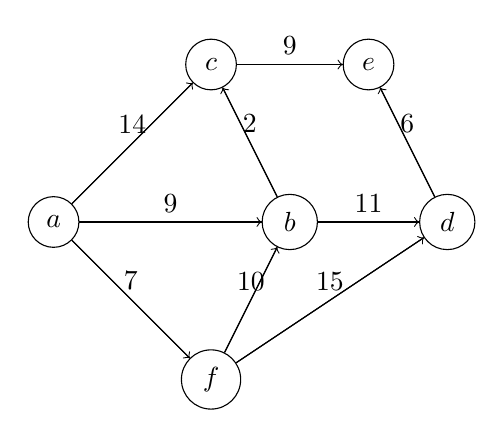
\begin{tikzpicture}
            \tikzset{
                vertex/.style={draw, circle, text width=8, align=center},arc/.style={->}
            }
            \draw node[vertex] (a) at (0,0) {$a$};
            \draw node[vertex] (b) at (3,0) {$b$};
            \draw node[vertex] (c) at (2,2) {$c$};
            \draw node[vertex] (d) at (5,0) {$d$};
            \draw node[vertex] (e) at (4,2) {$e$};
            \draw node[vertex] (f) at (2,-2) {$f$};		
            \foreach \x/\y in {%
            a/f, a/c,a/b,b/c,b/d,c/e,d/e,f/b,f/d%
            }{
                \draw (\x) edge[arc] (\y);
            }
            \draw[-] (a) -- node[above] {9} (b);
            \draw[-] (a) -- node[above] {14} (c);
            \draw[-] (a) -- node[above] {7} (f);
            \draw[-] (b) -- node[above] {11} (d);
            \draw[-] (b) -- node[above] {2} (c);
            \draw[-] (c) -- node[above] {9} (e);
            \draw[-] (d) -- node[above] {6} (e);
            \draw[-] (f) -- node[above] {15} (d);
            \draw[-] (f) -- node[above] {10} (b);
        \end{tikzpicture}
    \end{center}

	\begin{soln}
        % write your solution here

    \end{soln}
\end{prob}
